\begin{figure}
\setlength{\tabcolsep}{0.5pt}
    \centering
    { \small 
\begin{tabular}{ccccc}
Original & w/o e4e & w/o PTI & w/o Stitching & Ours \\
\raisebox{-.32\totalheight}{
\includegraphics[width=0.2\columnwidth]{resources/images/ablation_micheal/original/source_0100.jpeg}} &
\raisebox{-.32\totalheight}{
\includegraphics[width=0.2\columnwidth]{resources/images/ablation_micheal/no_e4e/optimized_0100.jpeg}} &
\raisebox{-.32\totalheight}{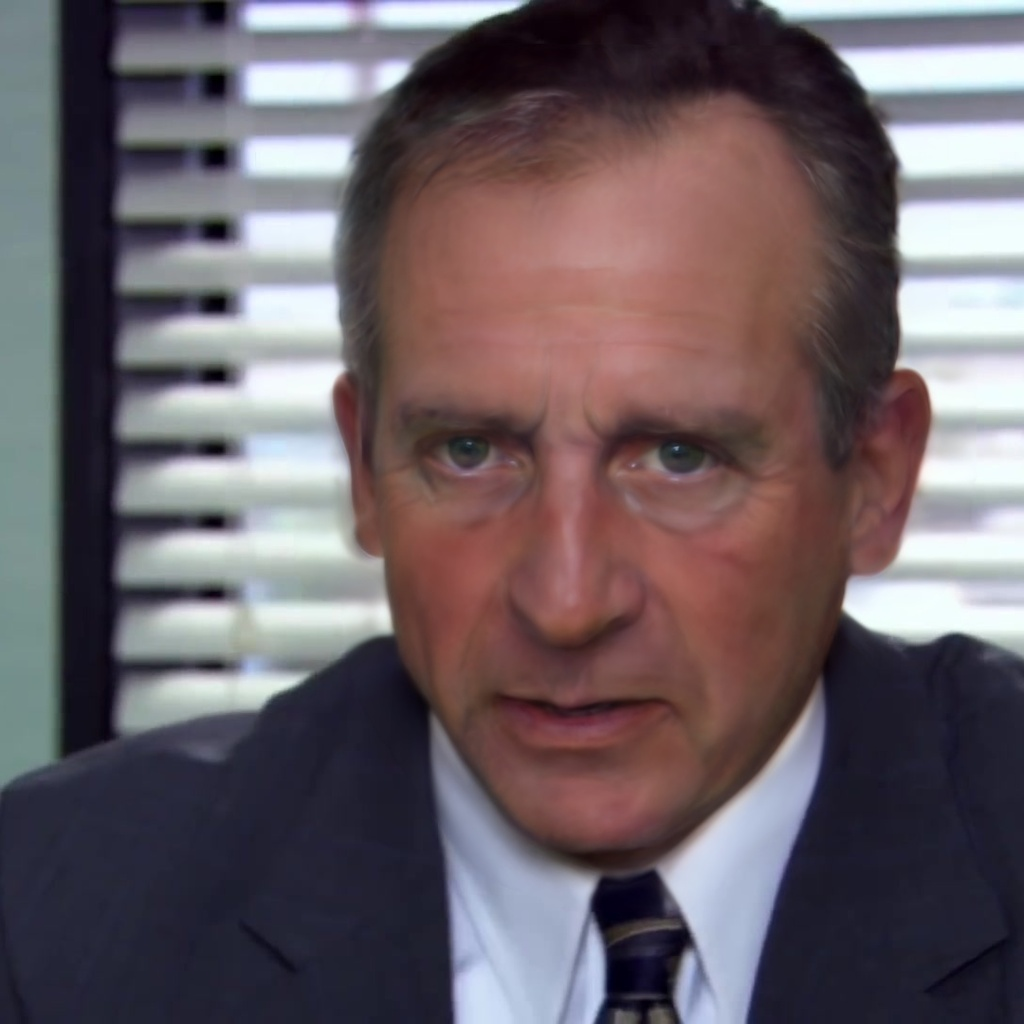
\includegraphics[width=0.2\columnwidth]{resources/images/ablation_micheal/no_pti/optimized_0100.jpeg}} &
\raisebox{-.32\totalheight}{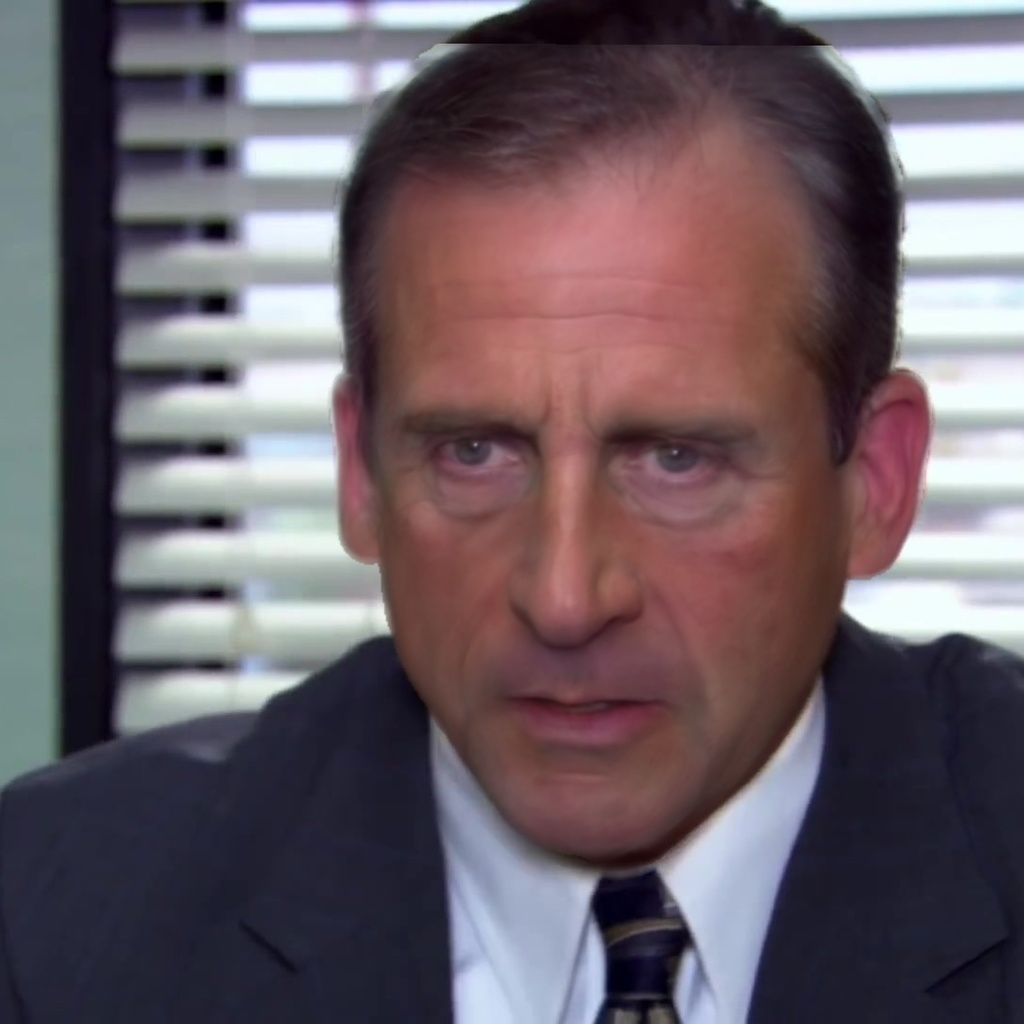
\includegraphics[width=0.2\columnwidth]{resources/images/ablation_micheal/no_stitching/edit_0100.jpeg}} &
\raisebox{-.32\totalheight}{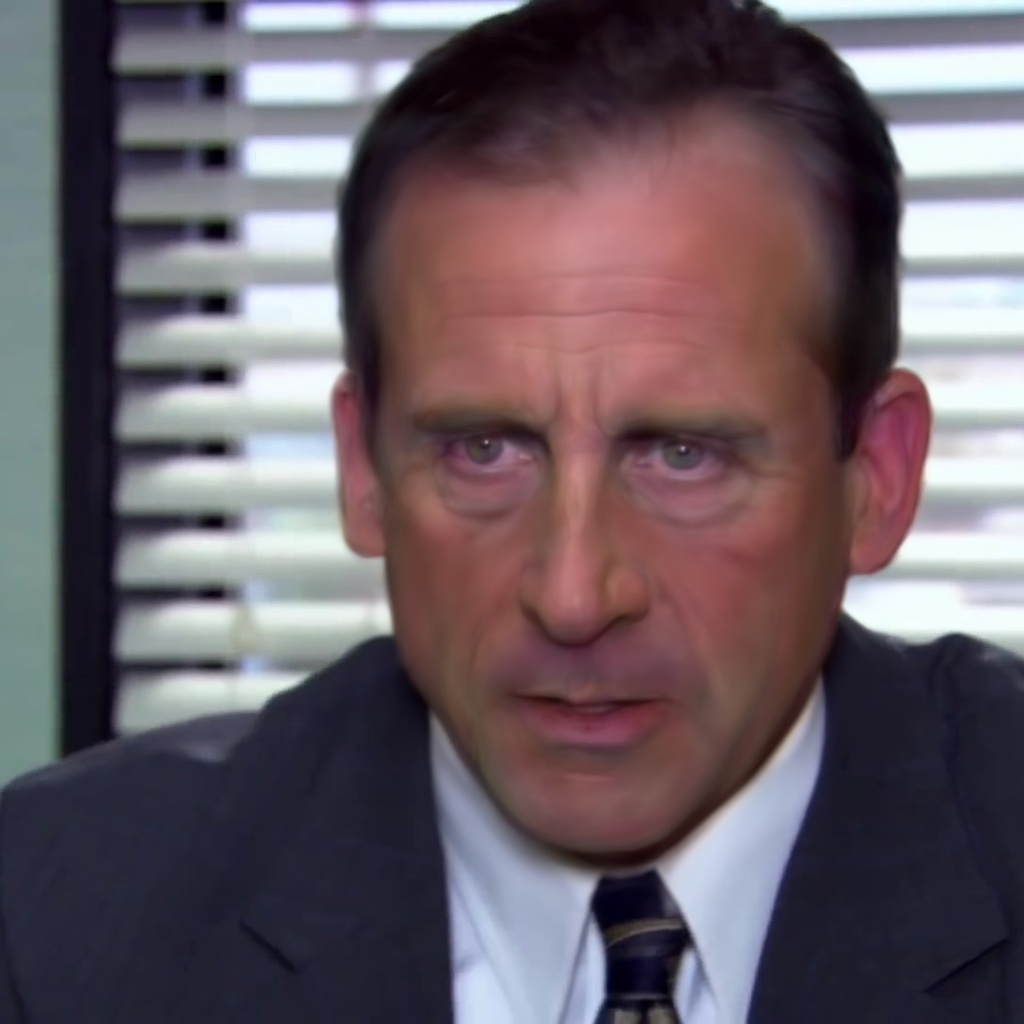
\includegraphics[width=0.2\columnwidth]{resources/images/ablation_micheal/ours/optimized_0100.jpeg}} \\

\raisebox{-.32\totalheight}{
\includegraphics[width=0.2\columnwidth]{resources/images/ablation_micheal/original/source_0083.jpeg}} &
\raisebox{-.32\totalheight}{
\includegraphics[width=0.2\columnwidth]{resources/images/ablation_micheal/no_e4e/optimized_0083.jpeg}} &
\raisebox{-.32\totalheight}{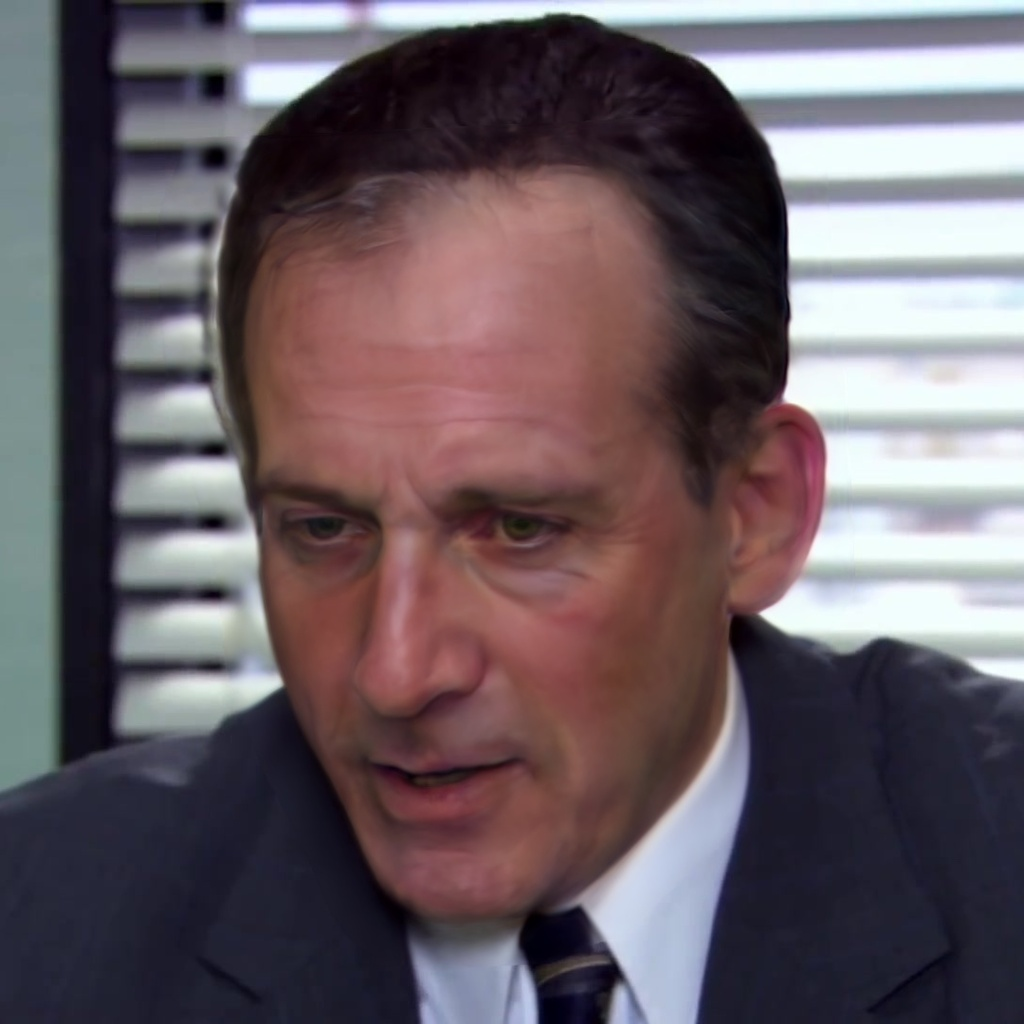
\includegraphics[width=0.2\columnwidth]{resources/images/ablation_micheal/no_pti/optimized_0083.jpeg}} &
\raisebox{-.32\totalheight}{
\includegraphics[width=0.2\columnwidth]{resources/images/ablation_micheal/no_stitching/edit_0083.jpeg}} &
\raisebox{-.32\totalheight}{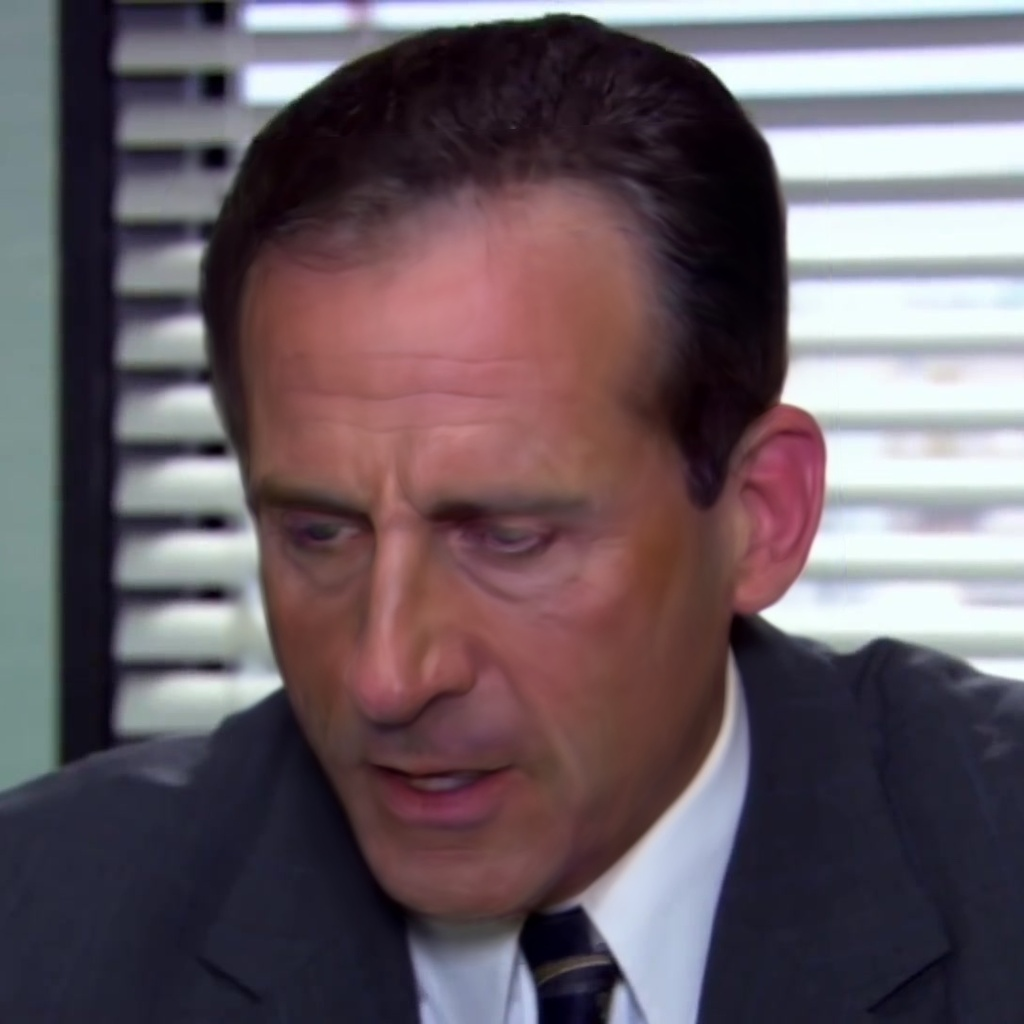
\includegraphics[width=0.2\columnwidth]{resources/images/ablation_micheal/ours/optimized_0083.jpeg}} \\

\raisebox{-.32\totalheight}{
\includegraphics[width=0.2\columnwidth]{resources/images/ablation_micheal/original/source_0030.jpeg}} &
\raisebox{-.32\totalheight}{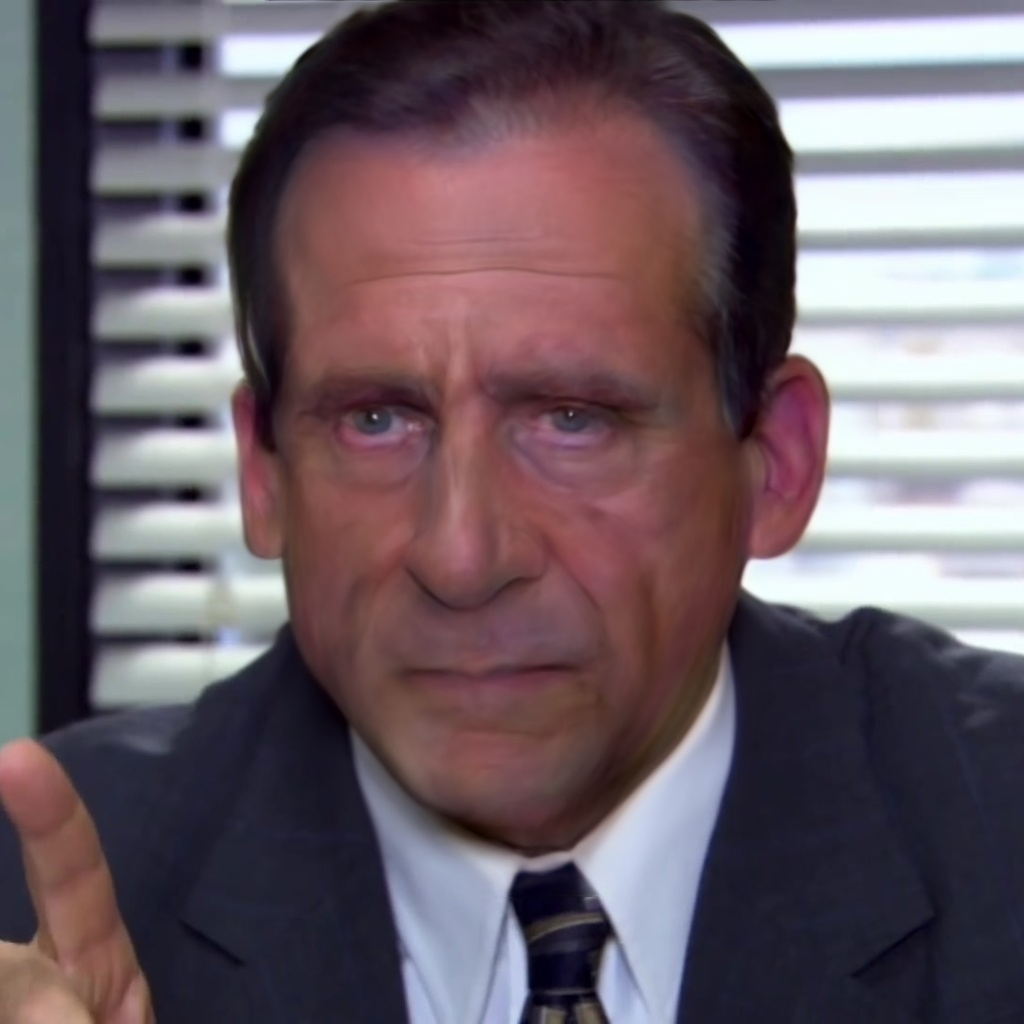
\includegraphics[width=0.2\columnwidth]{resources/images/ablation_micheal/no_e4e/optimized_0030.jpeg}} &
\raisebox{-.32\totalheight}{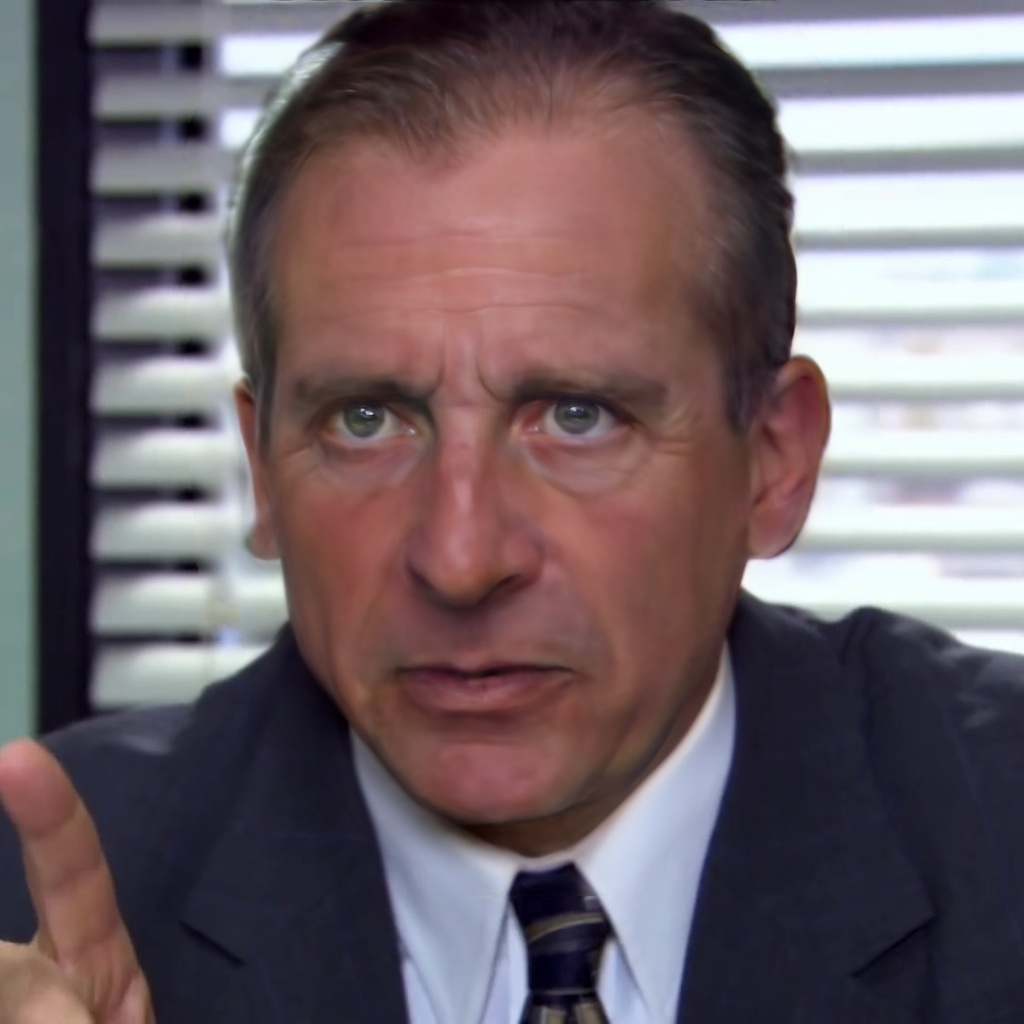
\includegraphics[width=0.2\columnwidth]{resources/images/ablation_micheal/no_pti/optimized_0030.jpeg}} &
\raisebox{-.32\totalheight}{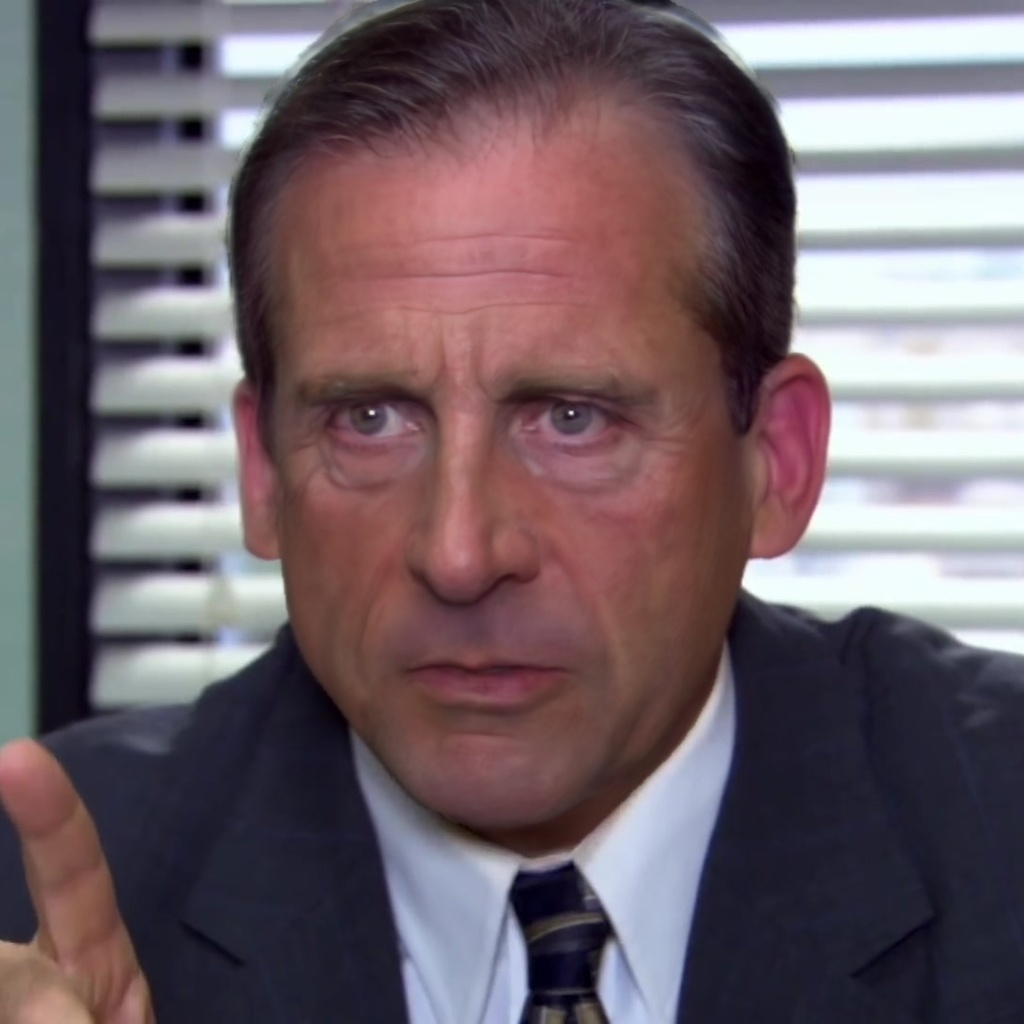
\includegraphics[width=0.2\columnwidth]{resources/images/ablation_micheal/no_stitching/edit_0030.jpeg}} &
\raisebox{-.32\totalheight}{
\includegraphics[width=0.2\columnwidth]{resources/images/ablation_micheal/ours/optimized_0030.jpeg}} \\

\raisebox{-.32\totalheight}{
\includegraphics[width=0.2\columnwidth]{resources/images/ablation_micheal/original/source_0000.jpeg}} &
\raisebox{-.32\totalheight}{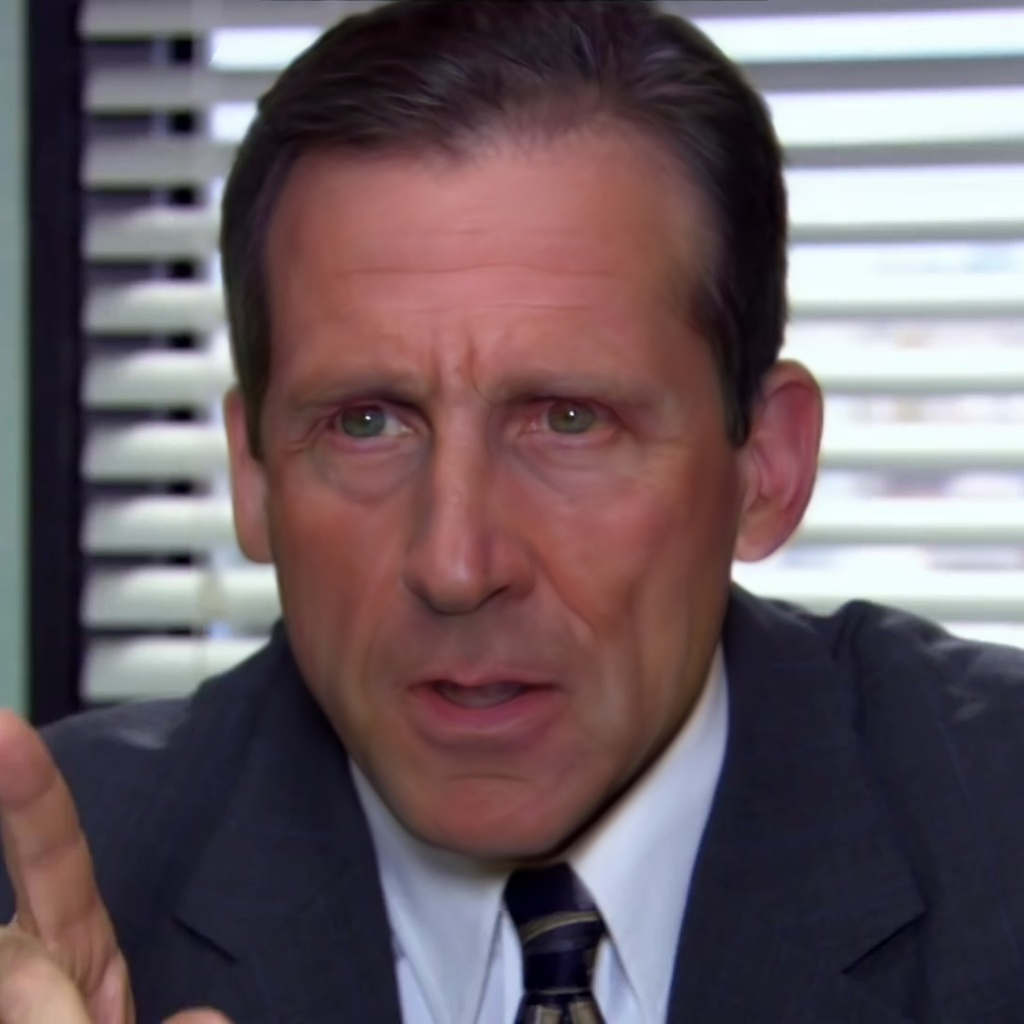
\includegraphics[width=0.2\columnwidth]{resources/images/ablation_micheal/no_e4e/optimized_0000.jpeg}} &
\raisebox{-.32\totalheight}{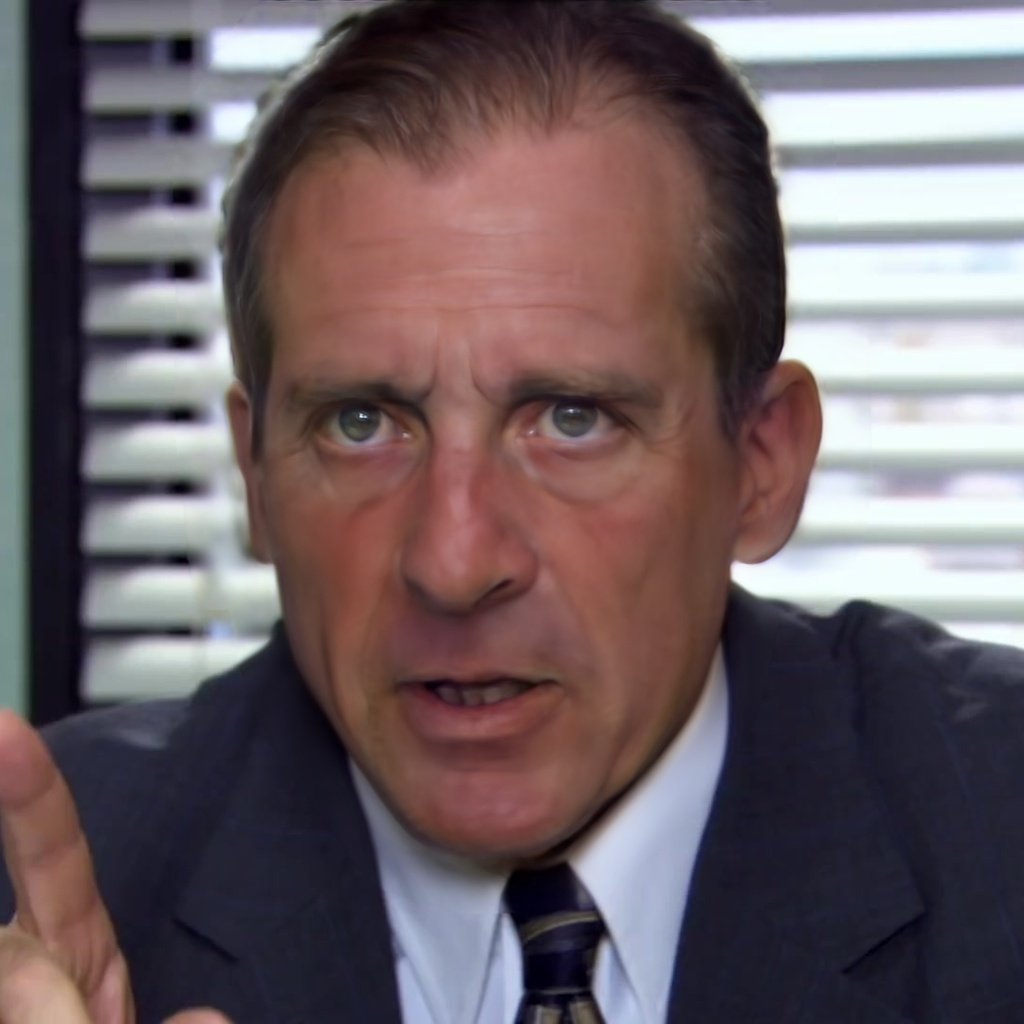
\includegraphics[width=0.2\columnwidth]{resources/images/ablation_micheal/no_pti/optimized_0000.jpeg}} &
\raisebox{-.32\totalheight}{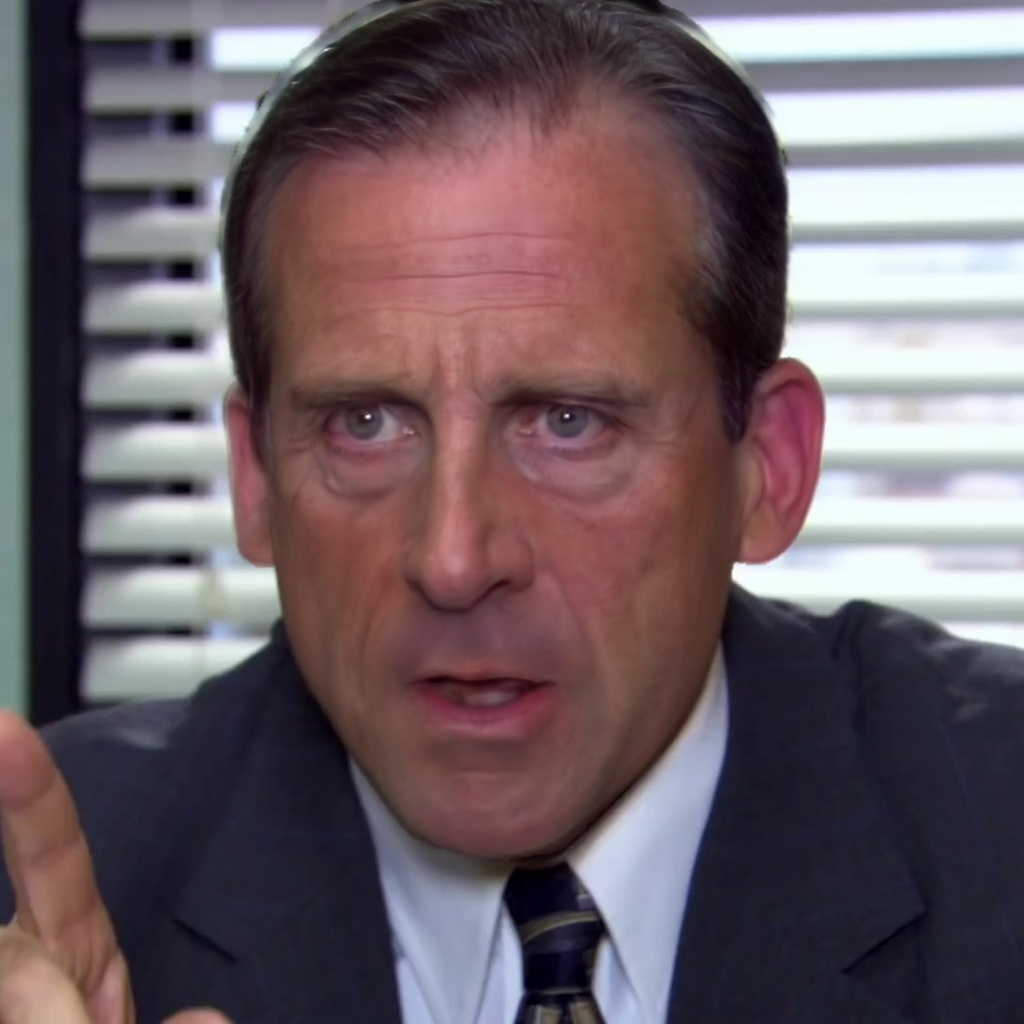
\includegraphics[width=0.2\columnwidth]{resources/images/ablation_micheal/no_stitching/edit_0000.jpeg}} &
\raisebox{-.32\totalheight}{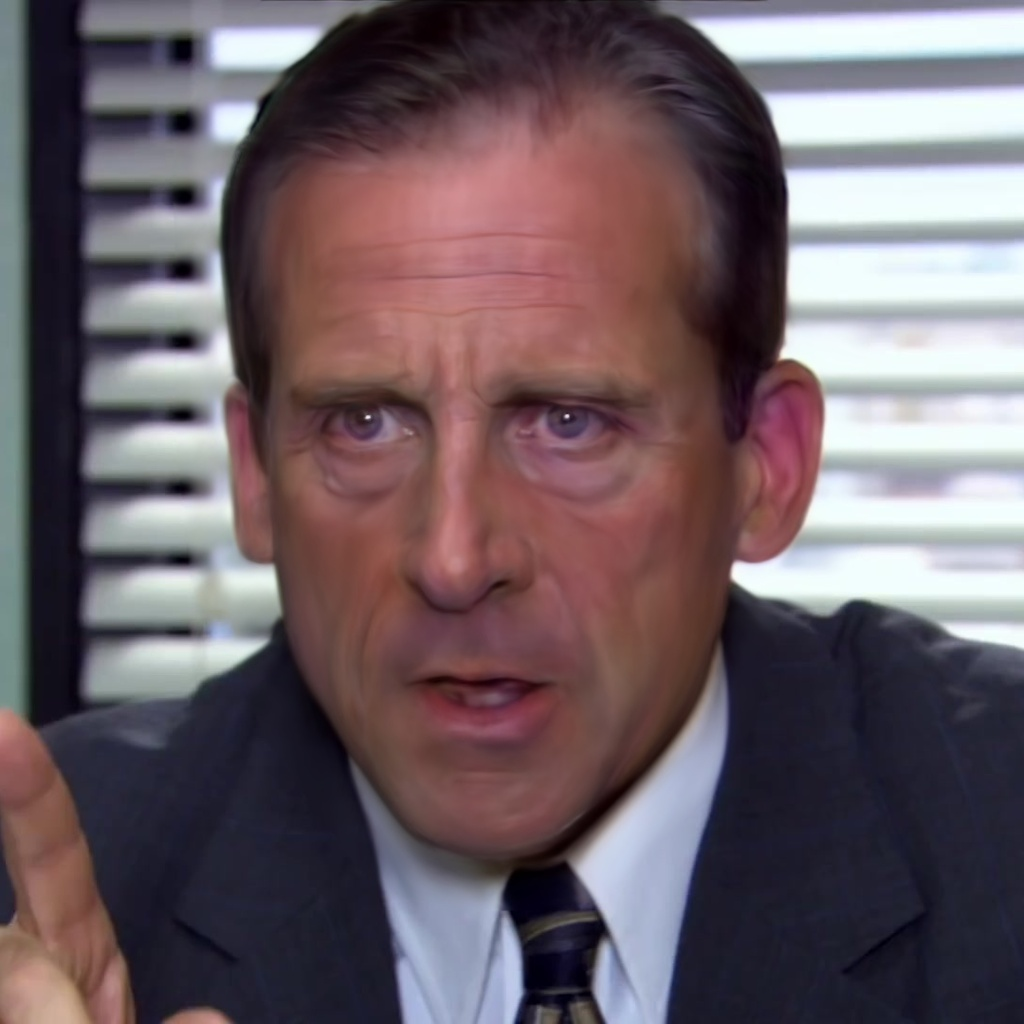
\includegraphics[width=0.2\columnwidth]{resources/images/ablation_micheal/ours/optimized_0000.jpeg}} \\

\end{tabular}
}


\caption{Qualitative demonstration of the importance of our pipeline components. Replacing the encoder with an optimization step results in poor editing consistency. Without PTI, identity drifts over time, and stitching performance deteriorates. Replacing stitching with a mask-based blending scheme results in visual artifacts, such as sharp transitions in hair regions. Our full pipeline successfully avoids these pitfalls and generates a consistent video.}
\label{fig:ablation}
\end{figure}